\section{Hall effect sensor (Digital)}
\begin{figure}[H]
    \centering
    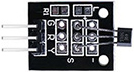
\includegraphics[angle=0, keepaspectratio=true, scale=1, width=200px, height=200px]{images/halleffect_digital.jpg}
    %\caption{Caption}
\end{figure}
\subsection*{Description}
This module is used to detect the prescence of an external magnetic field and has a digital output only.
\subsection*{Pin mapping}
This pin mapping corresponds to the pins from left to right with the module pins facing towards you.
\begin{table}[H]
    \centering
    \begin{tabular}{|c|c|c|c|c|}
    \hline
    Index &Label &Type &Name &Description\\ \hline
    0 &- &Ground &GND &Ground\\ \hline
    1 & &Source voltage &$V+$ &Module source voltage ($3.3V - 5V$)\\ \hline
    2 &S &Digital output &D0 &Hall effect sensor output\\ \hline
    \end{tabular}
    %\caption{Caption}
    %\label{tab:my_label}
\end{table}
\subsection*{Operation}
The digital output pin (D0) is high in the presence of no magnetic field. When a magnetic field is detected D0 is set to low. The sensor can only detect a magnetic field in one direction so try reversing the magnet if the output is not changing.
%\subsection*{Code}
%\lstinputlisting[caption=test]{laser.py}